\documentclass[notes, 10pt, aspectratio=169]{beamer}

\usepackage{pgfpages}
% These slides also contain speaker notes. You can print just the slides,
% just the notes, or both, depending on the setting below. Comment out the want
% you want.
\setbeameroption{hide notes} % Only slide
%\setbeameroption{show only notes} % Only notes
%\setbeameroption{show notes on second screen=right} % Both
\usepackage{helvet}
\usepackage[default]{lato}
\usepackage{array}
\usepackage{tikz}
\usepackage{verbatim}
\usepackage{natbib}
\bibliographystyle{apalike}
%\usepackage[affil-it]{authblk}
\tikzset{>=latex} % for LaTeX arrow head
\usepackage{pgfplots} % for the axis environment
\pgfplotsset{compat=1.18}
\usepackage{xcolor}
\usepackage{adjustbox}
\usepackage[outline]{contour} % halo around text
\setbeamertemplate{note page}{\pagecolor{yellow!5}\insertnote}
\contourlength{1.2pt}
\usepackage{amsmath}
\usepackage{newpxtext}
\usepackage[osf]{mathpazo}
\usepackage{hyperref}
\usepackage[pdf]{pstricks}
\usepackage{epstopdf}
\epstopdfsetup{update}
\usepackage{multimedia}
\usepackage{multirow}
\usepackage{dcolumn}
\usepackage{animate}
\usepackage{bbm}
\usepackage{booktabs}
\usepackage{blindtext}

\newcolumntype{d}[0]{D{.}{.}{5}}

\usepackage{changepage}
\usepackage{appendixnumberbeamer}
\newcommand{\beginbackup}{
	\newcounter{framenumbervorappendix}
	\setcounter{framenumbervorappendix}{\value{framenumber}}
	\setbeamertemplate{footline}
	{
		\leavevmode%
		\hline
		box{%
			\begin{beamercolorbox}[wd=\paperwidth,ht=2.25ex,dp=1ex,right]{footlinecolor}%
				%         \insertframenumber  \hspace*{2ex} 
		\end{beamercolorbox}}%
		\vskip0pt%
	}
}
\newcommand{\backupend}{
	\addtocounter{framenumbervorappendix}{-\value{framenumber}}
	\addtocounter{framenumber}{\value{framenumbervorappendix}} 
}

\usepackage{graphicx}
\usepackage[space]{grffile}
\usepackage{booktabs}

\definecolor{razorbackred}{RGB}{161,0,47}
\definecolor{appleblossom}{RGB}{255,255,255}
\definecolor{cardinalred}{RGB}{210,30,40}
\definecolor{springwater}{RGB}{62,148,170}
\definecolor{pine}{RGB}{60,110,60}
\definecolor{goldenoak}{RGB}{219,182,37}
\definecolor{hickory}{RGB}{157,34,53}
\definecolor{spoofers}{RGB}{70,70,72}


\renewcommand*{\bibfont}{\scriptsize}
\hypersetup{
	colorlinks=false,
	linkbordercolor = {white},
	linkcolor = {blue}
}

% define gaussian pdf and cdf
\pgfmathdeclarefunction{gauss}{3}{%
  \pgfmathparse{1/(#3*sqrt(2*pi))*exp(-((#1-#2)^2)/(2*#3^2))}%
}
\pgfmathdeclarefunction{cdf}{3}{%
  \pgfmathparse{1/(1+exp(-0.07056*((#1-#2)/#3)^3 - 1.5976*(#1-#2)/#3))}%
}
\pgfmathdeclarefunction{fq}{3}{%
  \pgfmathparse{1/(sqrt(2*pi*#1))*exp(-(sqrt(#1)-#2/#3)^2/2)}%
}
\pgfmathdeclarefunction{fq0}{1}{%
  \pgfmathparse{1/(sqrt(2*pi*#1))*exp(-#1/2))}%
}
\colorlet{mydarkblue}{blue!30!black}


%% I use a beige off white for my background
\definecolor{MyBackground}{RGB}{255,253,218}

%% Uncomment this if you want to change the background color to something else
%\setbeamercolor{background canvas}{bg=MyBackground}

%% Change the bg color to adjust your transition slide background color!
\newenvironment{transitionframe}{
	\setbeamercolor{background canvas}{bg=yellow}
	\begin{frame}}{
	\end{frame}
}

\setbeamercolor{frametitle}{fg=cardinalred}
\setbeamercolor{title}{fg=black}
\setbeamertemplate{footline}[frame number]
\setbeamertemplate{navigation symbols}{} 
\setbeamertemplate{itemize items}{-}
\setbeamercolor{itemize item}{fg=razorbackred}
\setbeamercolor{itemize subitem}{fg=pine}
\setbeamercolor{enumerate item}{fg=springwater}
\setbeamercolor{enumerate subitem}{fg=spoofers}
\setbeamercolor{button}{bg=MyBackground,fg=blue,}
\setbeamercolor{block title}{bg=springwater,fg=spoofers}
\setbeamercolor{section in toc}{fg=blue}
\setbeamercolor{subsection in toc}{fg=red}
\setbeamersize{text margin left=1em,text margin right=1em} 
%\setbeamertemplate{footline}{\hspace*{.5cm}\scriptsize{\insertauthor
%\hspace*{50pt} \hfill\insertframenumber\hspace*{-5cm}}}
%\setbeamertemplate{footline}[frame number]
\setbeamertemplate{page number in head/foot}{}

\newenvironment{wideitemize}{\itemize\addtolength{\itemsep}{10pt}}{\enditemize}

\usepackage{environ}
\NewEnviron{videoframe}[1]{
	\begin{frame}
		\vspace{-8pt}
		\begin{columns}[onlytextwidth, T] % align columns
			\begin{column}{.58\textwidth}
				\begin{minipage}[t][\textheight][t]
					{\dimexpr\textwidth}
					\vspace{8pt}
					\hspace{4pt} {\Large \sc \textcolor{blue}{#1}}
					\vspace{8pt}
					
					\BODY
				\end{minipage}
			\end{column}%
			\hfill%
			\begin{column}{.42\textwidth}
				\colorbox{green!20}{\begin{minipage}[t][1.2\textheight][t]
						{\dimexpr\textwidth}
						Face goes here
				\end{minipage}}
			\end{column}%
		\end{columns}
	\end{frame}
}

\title[]{\textcolor{razorbackred}{Crop Rotations, Transition Costs,
and Farm Delinquencies}\\
\small \textit{Why rotation protects the farm balance sheet, even when price risk dominates revenue variance}}
\author[]{Victor Funes-Leal\inst{1} \and Lawson Connor\inst{1} \and Eunchun Park\inst{1}}
\institute[]{\inst{1} Department of Agricultural Economics and Agribusiness, University of Arkansas}
\date{}

 
\makeatletter

\begin{document}

% logo of my university  
%\logo{
\includegraphics[width=2.5cm]{figures/ACES-Logo.pdf}}
\titlegraphic { 
\begin{tikzpicture}[overlay,remember picture]
\node[right = 0.2cm] at (current page.200){
    
\includegraphics[scale = 0.15]{figs/UA_Logo.eps}
};
\end{tikzpicture}
}
	
	%%% TIKZ STUFF
	\tikzset{   
		every picture/.style={remember picture,baseline},
		every node/.style={anchor=base,align=center,outer sep=1.5pt},
		every path/.style={thick},
	}
	\newcommand\marktopleft[1]{%
		\tikz[overlay,remember picture] 
		\node (marker-#1-a) at (-.3em,.3em) {};%
	}
	\newcommand\markbottomright[2]{%
		\tikz[overlay,remember picture] 
		\node (marker-#1-b) at (0em,0em) {};%
	}
	\tikzstyle{every picture}+=[remember picture] 
	\tikzstyle{mybox} =[draw=black, very thick, rectangle, inner sep=10pt, inner ysep=20pt]
	\tikzstyle{fancytitle} =[draw=black,fill=red, text=white]
	%%%% END TIKZ STUFF

% ----- Geometry -----
% Slide aspect: 13.333 x 7.5 in. We scale TikZ coordinates to cm.
\newcommand{\boxwidth}{4.0cm}
\newcommand{\boxheight}{1.8cm}
\newcommand{\boxgap}{1.4cm}     % horizontal gap between component boxes
\newcommand{\outputw}{14.6cm}   % wide enough to hold the full output line
\newcommand{\outputh}{1.3cm}
 
	% Title Slide
 
\begin{frame}
	\maketitle
	\centering 
    
\end{frame}

%\begin{frame}{Motivation}
%\begin{block}{Operating credit is the financial lifeline of row-crop farms.}
%\begin{wideitemize}
%    \item Farmers borrow against planting, accrue interest through the growing season, and retire the balance at harvest.
%    \item When revenue falls short, the unpaid balance \textbf{rolls forward}, compounding at a contractual rate and enlarging next spring's principal.
%\end{wideitemize}
%\end{block}

%\begin{block}{Compounding Chain}
%    \begin{description}
%        \item[Year $t$]: bad harvest $\rightarrow$ unpaid balance \$B.
%        \item[Year $t+1$]: principal grows to \$ $B(1+r)+$ new spring loan.
%        \item[Year $t+2$]: prior shock still in principal: default risk increases.
%        \item[Year $t+k$]: small initial shock $\rightarrow$ delinquency
%    \end{description}
%\end{block}
%\end{frame}

%\begin{frame}{Motivation}
%    \small
%    \begin{block}{Climate Pressure}
%        \begin{itemize}
%            \item US Midwest corn \& soy yield: -7-9\% projected by 2050 (drought + heat)
%            \item Extreme heat $+$ dry spells to co-occur more $\rightarrow$ yield shock variance $\uparrow$.
%        \end{itemize}
%    \end{block}
%    \begin{block}{Global Competitor Expansion}
%        \begin{itemize}
%            \item Brazil now 58\% of global soy exports; US share fell to 28\% (2024/25 USDA).
%            \item US soy exports to China: 60\% avg. pre-trade-war $\rightarrow$ 47\% post (2018–2024).
%            \item Brazil corn exports surging — filling gaps left by Ukraine war disruption.
%            \item Chronic price pressure on US corn-soy revenue $\rightarrow$ thinner debt-repayment margins.
%        \end{itemize}
%    \end{block}
%    \begin{block}{Land \& Input Competition}
%        \begin{itemize}
%            \item Data centers $+$ solar: 1M+ acres of farmland converted; 70\% of solar in Midwest on cropland.
%            \item Farm electricity costs $\uparrow 48\%$ projected 2019–2026 (USDA ERS).
%        \end{itemize}
%    \end{block}
%\end{frame}

\begin{frame}{Motivation}
    \begin{columns}[T] % align columns
    \begin{column}{.55\textwidth}
    \resizebox{\textwidth}{!}{
        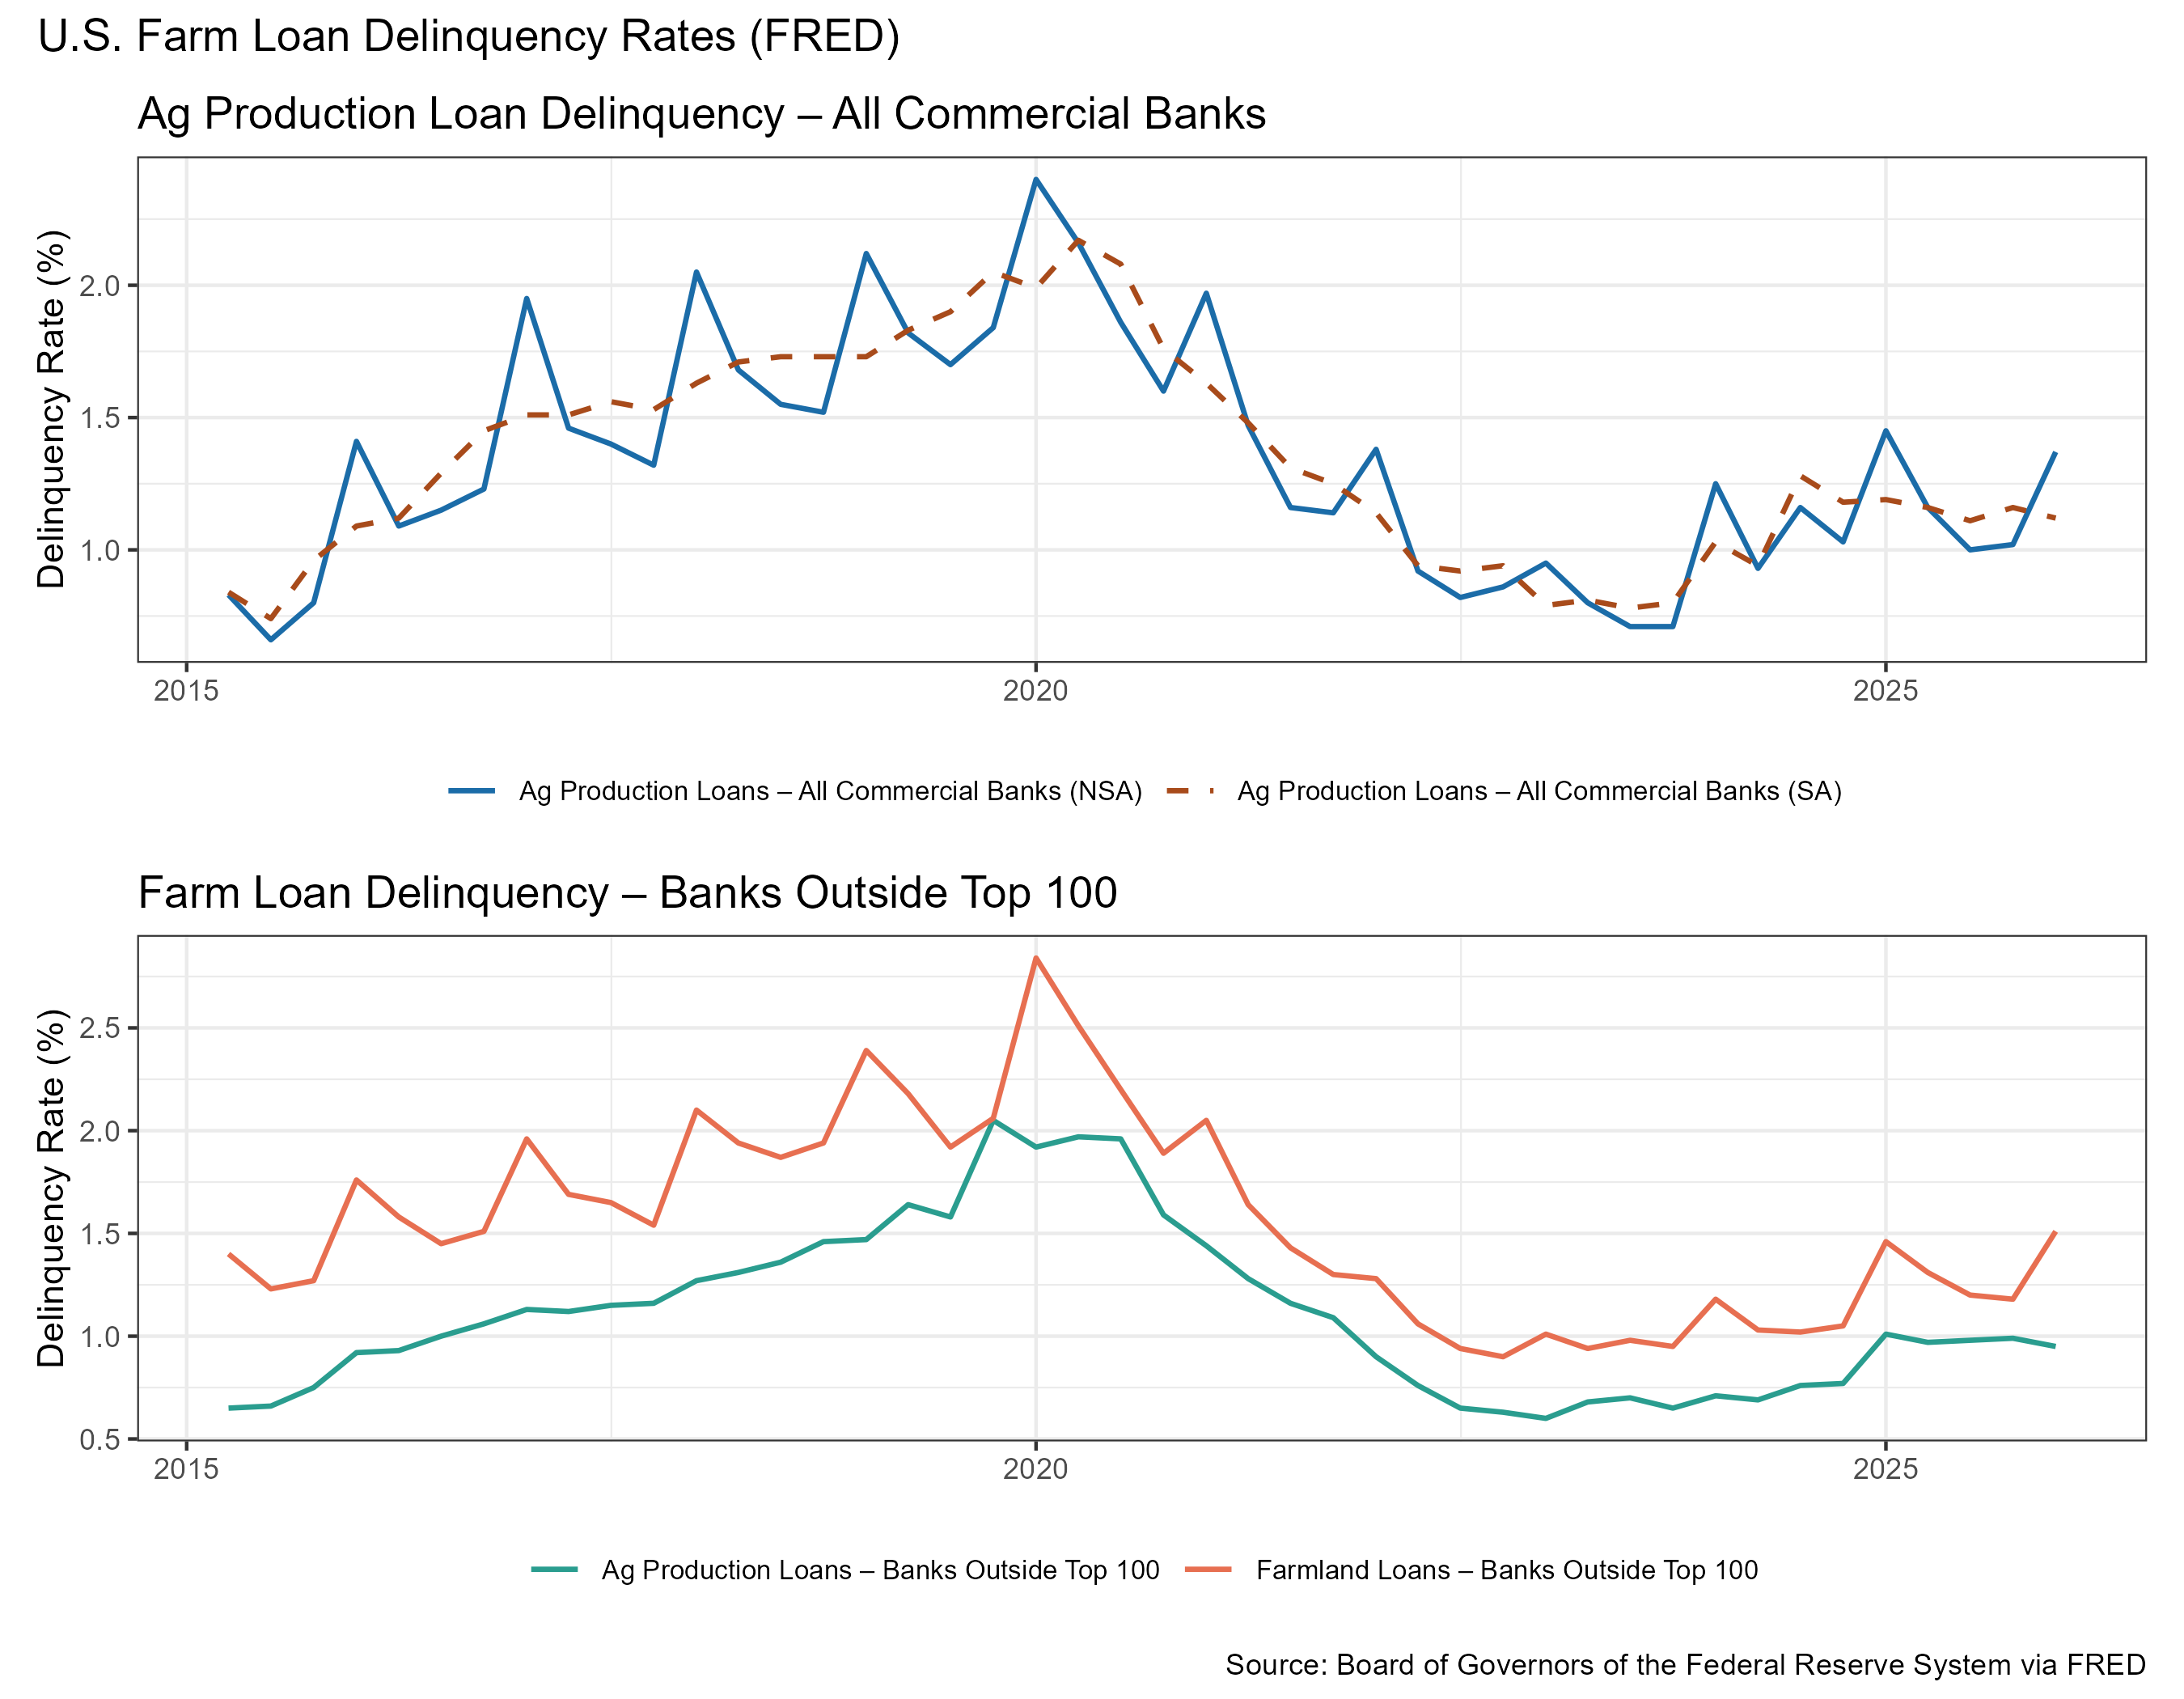
\includegraphics{figs/fred_farm_delinquency_plot.png}
    }
    \footnotesize
    These shocks operate through prices. This paper quantifies how rotation history shapes the path from price shock to delinquency.
    \end{column}%
    \hfill%
    \begin{column}{.45\textwidth}
    \begin{itemize}
    %\item \textcolor{cardinalred}{2015-16} \textbf{Commodity price collapse}: Corn falls from \$7 $\rightarrow$ \$3.50/bu. Farm income drops by 45\% over 3 years. Operating-loan stress builds.
    %\item \textcolor{springwater}{2018-19} \textbf{US-China trade war}: Soy exports to China collapse. U.S. world soy export share falls from 38\% $\rightarrow$ 28\% as Brazil captures the gap.
    \item \textcolor{pine}{2020} \textbf{COVID + CFAP payments}: Delinquency spikes to 2.3\% (peak). CFAP/ARC-CO transfers temporarily mask rollover risk through 2021. 
    \item \textcolor{hickory}{2022} \textbf{Russia–Ukraine war}: Wheat/corn price spike then collapse. Ukraine recovers export corridor; Black Sea grain competes again by 2023.
    \item \textcolor{goldenoak}{2024-} \textbf{Second uptick underway}: NSA rate at 1.4\% and climbing. Iran–Israel tensions and U.S. export-share erosion sustain pressure.
  \end{itemize}
\end{column}%
\end{columns}
\end{frame}

\begin{frame}{Research questions}
    \begin{wideitemize}
        \item \textcolor{red}{\textbf{Question 1}}: What is the net benefit of complex rotation after accounting for alternative revenue hedging options?
        \item \textcolor{red}{\textbf{Question 2}}: How can we estimate delinquency probabilities conditioning on yields on the full six-year rotation history of the field?
        \item \textcolor{red}{\textbf{Question 3}}: How does the negative price–yield correlation change those probabilities, and do its effects act as a substitute for or complement to rotation?
        \item If revenue is treated as one aggregate stream and default is predicted from one-year loss probabilities, crop rotation effects are not accounted for.
        \item \textbf{Sustainable practices}: We show that, crop rotation reduces the debt-rollover chain, and lowers multi-year delinquency risk. It is the link between agronomic sustainability and financial resilience.
    \end{wideitemize}
\end{frame}

\begin{frame}{Contributions to literature}
\begin{block}{Rotation agronomy: Yields condition on prior crops}
    \begin{itemize}
        \item \textit{Key Papers}: \cite{Bullock1992, Seifert2017}
        \item \textit{What's missing}: Strictly yield modeling. No financial channel.
    \end{itemize}
\end{block}

\begin{block}{Dynamic crop choice: Optimal sequential planting}
    \begin{itemize}
        \item \textit{Key Papers}: \cite{Burt1963, Livingston2015, Chen2025}
        \item \textit{What's missing}: Optimal policy, not policy-conditional survival.
    \end{itemize}
\end{block}

\begin{block}{Farm credit risk: Farm survival and exit decisions}
    \begin{itemize}
        \item \textit{Key Papers}: \cite{Featherstone1988, Ifft2015, Kim2020, Lee2024}
        \item \textit{What's missing}: Yield as a single aggregate. No rotation state.
    \end{itemize}
\end{block}

This article: couple rotation-conditioned yields with an explicit operating-credit cash-flow process $\rightarrow$ multi-year delinquency.
\end{frame}

\begin{frame}{Data}
We use a field-level panel that covers the entire state of Illinois from 2008 to 2022.

\begin{description}
    \item[Yields]: Quantitative Domain Adversarial Neural Networks (QDANN), \cite{Ma2024}, satellite-derived yield maps for every field-year.
    \item[Rotations]: Cropland Data Layer (CDL), full six-year crop history.
    \item[Weather]: GRIDMET \citep{Abatzoglou2013} + TerraClimate \citep{Abatzoglou2018}, growing-season vapor-pressure deficit (VPD), Palmer Drought Severity Index (PDSI).
    \item[Soil]: gSSURGO, NCCPI productivity index per field.
    \item[IL Regions]: Illinois Farm Business Farm Management/Farmdoc definition (North, Central, South).
    \item[Productivity zones]: Empirical tertiles of average yields by region.
\end{description}
\end{frame}

% ============================================================
%  Framework diagram as a 16:9 beamer frame
%  Compile with: pdflatex framework_beamer.tex
%  Slide size: 16:9 (159.2 mm x 89.55 mm content area, beamer default for 169)
% ============================================================
%\documentclass[aspectratio=169,11pt]{beamer}

% ----- Plain / clean theme (no Madrid/Warsaw decoration) -----
%\usetheme{default}
%\usecolortheme{default}
%\beamertemplatenavigationsymbolsempty   % no navigation icons
%\setbeamertemplate{footline}{}          % no footer bar
%\setbeamertemplate{headline}{}          % no header bar
%\setbeamertemplate{frametitle continuation}{}

% ----- Fonts: serif for headers + sans for body (matches the talk) -----
%\usepackage[T1]{fontenc}
%\usepackage{microtype}
%\usepackage{charter}                    % serif for headings (Lora stand-in)
%\usepackage[scaled=0.92]{helvet}        % sans for body     (Carlito stand-in)
%\renewcommand{\familydefault}{\sfdefault}

% ----- Packages -----
%\usepackage{xcolor}
%\usepackage{tikz}
%\usepackage{varwidth}
\usetikzlibrary{arrows.meta, positioning, calc}

% ----- Palette (same hex values as the .pptx) -----
\definecolor{ink}{HTML}{1B1C19}
\definecolor{paper}{HTML}{FFFFFF}
\definecolor{muted}{HTML}{585B52}
\definecolor{rule}{HTML}{C9C2AA}
\definecolor{corn}{HTML}{C0392B}        % operating credit
\definecolor{mix}{HTML}{D99A2B}         % price-yield copula
\definecolor{soy}{HTML}{3F7233}         % yield generator
\definecolor{soydeep}{HTML}{2A4D22}     % output banner
\definecolor{soysoft}{HTML}{C9D9BD}     % "Output:" label color

% ----- Beamer styling: clean frame title + minimal margins -----
%\setbeamercolor{frametitle}{fg=ink, bg=paper}
%\setbeamerfont{frametitle}{family=\rmfamily, series=\bfseries, size=\Large}
%\setbeamertemplate{frametitle}{%
  %\vspace{0.35em}%
  %\hspace{0.10em}%
%  \begin{varwidth}{0.95\paperwidth}
%    {\sffamily\bfseries\fontsize{8.5}{10}\selectfont\color{soydeep}%
%     S\,I\,M\,U\,L\,A\,T\,I\,O\,N\ \ F\,R\,A\,M\,E\,W\,O\,R\,K}\par
    %\vspace{1mm}
%    \insertframetitle\par
    %\vspace{0.5mm}
%    {\sffamily\itshape\fontsize{10}{12}\selectfont\color{muted}%
%     Each component below is itself standard; the combination is new.}
%  \end{varwidth}%
%}

% ----- TikZ geometry (in cm) — sized for the 16:9 content area -----
% Content area is ~15.9 cm wide x ~8.9 cm tall; after frame title leaves
% roughly 5.5 cm of vertical room for the figure.
%\newcommand{\boxwidth}{3.6cm}
%\newcommand{\boxheight}{1.4cm}
%\newcommand{\boxgap}{1.0cm}
%\newcommand{\outputw}{12.8cm}            % spans under all three boxes
%\newcommand{\outputh}{1.05cm}

% ----- Component-box macro (defined at preamble level — beamer strips #
%       arguments if the macro is defined inside a frame) -----
% \compbox{name}{x-anchor (left edge)}{title}{subtitle}{color}
\newcommand{\compbox}[5]{%
  \begin{scope}
    % outer frame (colored border)
    \draw[#5, line width=1.3pt]
      (#2,0) rectangle ++(\boxwidth,-\boxheight);
    % colored top stripe
    \fill[#5] (#2,0) rectangle ++(\boxwidth,-0.08cm);
    % title
    \node[anchor=north west, text=ink] at ($(#2,0)+(0.28cm,-0.32cm)$) {%
      \rmfamily\bfseries\fontsize{12}{14}\selectfont #3};
    % subtitle (italic, muted)
    \node[anchor=north west, text=muted] at ($(#2,0)+(0.28cm,-0.90cm)$) {%
      \sffamily\itshape\fontsize{9.5}{11}\selectfont #4};
    % invisible anchors for arrows
    \coordinate (#1-east)  at ($(#2,0)+(\boxwidth, -\boxheight/2)$);
    \coordinate (#1-west)  at ($(#2,0)+(0,        -\boxheight/2)$);
    \coordinate (#1-south) at ($(#2,0)+(\boxwidth/2, -\boxheight)$);
    \coordinate (#1-north) at ($(#2,0)+(\boxwidth/2, 0)$);
  \end{scope}
}

%\begin{document}

\begin{frame}{Simulation framework}
\begin{block}{Three components, one cash-flow loop}
  \textit{Each component below is itself standard; the combination is new.}  
\end{block}
\vspace{1mm}
\begin{center}
\begin{tikzpicture}[
    every node/.style = {inner sep=0pt, outer sep=0pt},
    arrow/.style      = {-{Latex[length=2.2mm,width=1.8mm]}, line width=0.9pt, ink},
  ]
 
  % ---------- three component boxes ----------
  \compbox{yield}{0cm}%
    {Yield generator}{rotation-conditioned}{soy}
 
  \compbox{cop}%
    {\boxwidth + \boxgap}%
    {Price--yield copula}{decomposed correlation}{mix}
 
  \compbox{credit}%
    {2*\boxwidth + 2*\boxgap}%
    {Operating credit}{intra-year cash-flow}{corn}
 
  % horizontal arrows between boxes
  \draw[arrow] (yield-east) -- (cop-west);
  \draw[arrow] (cop-east)   -- (credit-west);
 
  % downward arrow from middle box to output banner
  \coordinate (mid-down-end) at ($(cop-south)+(0,-0.7cm)$);
  \draw[arrow] (cop-south) -- (mid-down-end);
 
  % ---------- output banner, centered under the three-box row ----------
  \coordinate (row-center) at ($(yield-north)!0.5!(credit-north)$);
  \coordinate (output-nw)  at ($(row-center)+(-\outputw/2,-\boxheight-0.75cm)$);
 
  \fill[soydeep] (output-nw) rectangle ++(\outputw,-\outputh);
 
  \node[anchor=west] at ($(output-nw)+(0.45cm,-\outputh/2)$) {%
    {\sffamily\bfseries\fontsize{12}{14}\selectfont\color{soysoft}Output:}%
    \hspace{0.4em}%
    {\sffamily\fontsize{11.5}{14}\selectfont\color{paper}%
     6-year delinquency probability per (region $\times$ zone $\times$ plan)}%
  };
 
\end{tikzpicture}
\end{center}

\end{frame}

%\end{document}


\begin{frame}{Simulation framework}
\begin{block}{Nonparametric conditional distribution $F_{Y|s,c,z}$}
    \begin{itemize}
        \item State s = 6-character rotation history (e.g., 'CSCSCS', 'CCCCCC') — up to 64 states per cell
        \item Two-way FE residuals: $y_{f,t} = \alpha_f + \gamma_t + \varepsilon_{f,t}$. Field FE removes permanent productivity; year FE removes common shocks. 
        \item Residual pool: $20,000$ bootstrap draws per state. (With replacement when $n < 20,000$).
        \item Simulation draws: $\overline{Y}=\mu(s)+\tilde{\varepsilon}$, where $\tilde{\varepsilon}\sim $ empirical residual pool.
        \item Deliberate nonparametric choice: continuous-corn lower tails may be fatter than Beta/Gamma would predict.
    \end{itemize}
\end{block}

\begin{block}{Lower-Tail Dominance}
    \begin{equation}
        F_{CS}(y)\leq F_{CC}(y)\,\text{ for all }y\leq\overline{y}(c,s)
    \end{equation}
    Verified in all $(c,s)$ cells at the 10$^{th}$ percentile
\end{block}
    
\end{frame}

\begin{frame}{Design: Financial side and plans}
    \begin{block}{Operating Credit Cycle}
        \begin{enumerate}
            \item \textit{Spring origination}: principal sized to planted crop.
            \item \textit{9-month accrual}: interest at contractual rate.
            \item \textit{Harvest repayment}: from realized revenue.
            \item \textit{Balance rollover}: shortfall compounds to next year
        \end{enumerate}
    \end{block}
\begin{block}{Three Plans}
  \begin{description}
  \item[CSCSCS]: Perfect corn/soy rotation (53\% prevalence).
  \item[CCCCCC]: Continuous corn (7\% prevalence).
  \item[CCSCCS]: Two corn/1 soy (6\% prevalence).
  \end{description}  
\end{block}    

\textbf{Key contrast}: CSCSCS and CCSCCS share the same two crops but differ in when soy first appears; that timing is the placebo lever we'll exploit later.
\end{frame}

\begin{frame}{The credit cycle: Operating loans cycle through the growing season}
\begin{columns}
    \begin{column}{0.48\linewidth}
      \begin{block}{Timing}
        \begin{description}
            \item[Jan] Planting $\rightarrow$ Borrow: $Cost_{t}+\text{carried debt}$
            \item[Feb-Sep] 9-month accrual: Debt$\times(1+r/12)^{9}$ at $r\approx 9\%$ APR
            \item[Oct] Harvest: $Revenue_{t}=Price_{t}\times Yield_{t}$
            \item[Oct] Repay: pay $\min\left(Revenue_{t}, Debt_{t}\right)$
            \item[Nov] Carry: shortfall rolls to the year $t+1$ principal
       \end{description}
      \end{block}
    \end{column}
    \begin{column}{0.48\linewidth}
      \begin{block}{Example: Year 2 (corn after corn)}
            \begin{tabular}{lc}
            \\
              Debt Carried in   &  \$/ac 50 \\
              Year 2 cost   &  \$/ac 630\\
              Principal needed   &  \$/ac 680 \\
              $\times$ growth factor $(1.0075)^{9}$ & 1.0696\\
              \textbf{Debt at harvest} & \$/ac 727\\
              \\
              Realized revenue & \$/ac 610\\
              $Payment = \min(rev,debt)$ & \$/ac 610\\
              \textbf{Carried to year 3} & \$/ac 117\\
              \\
              \\
            \end{tabular}
      \end{block}
    \end{column}
  \end{columns}
\textbf{Delinquency rule}: $remaining\_balance >0$ at year-end ("end-balance-positive"). Robustness: "over-limit" rule (balance $>$ credit ceiling). 
\end{frame}

\begin{frame}{The credit recursion}
    \begin{block}{Five equations define delinquency}
       \begin{enumerate}
        \item Spring origination: $L_{t} = C_{t} + B_{t-1}$
        \item Nine-month accrual: $H_{t} = L_{t}\times (1 + i)^{9/12}$
        \item Harvest revenue: $R_t = P_t\times Y_t$
        \item Repayment: $M_t = \min(R_t, H_t)$
        \item Carry forward $B_t = H_t - M_t\rightarrow \text{delinquency if } B_t > 0$
    \end{enumerate}
       A farm is delinquent if: $Debt\_carried_{t}>0$
    \end{block}
    \begin{block}{Why this recursion?}
        \small\begin{itemize}
            \item The simple-profit alternative is $Profit_{t} = P_{t}Y_{t} - Cost_{t}$; it sums to the same NPV but loses the path. 
            \item Eq. (5) is what carries the bad year forward: $shortfall \times (1+r)^{9/12}$ becomes next year's principal. A small year-1 shock can therefore compound into multi-year delinquency, the channel that current credit-risk models miss.
        \end{itemize}
    \end{block}
\end{frame}

%\begin{frame}{Decomposing yield shocks: aggregate vs idiosyncratic}
%      \begin{align*}
%          \text{Yield Shock} &= \text{\textcolor{razorbackred}{Aggregate risk}}+\text{\textcolor{springwater}{Idiosyncratic risk}}\\
%          Y_{it} &= (\alpha_{i}+\gamma_{t})+\varepsilon_{it}
%      \end{align*} 
%  \begin{description}
%    \item [Yield shock] Year-to-year deviation of a field's yield from its rotation-state mean — the part the farmer cannot predict at planting.
%      \item[\textcolor{razorbackred}{Aggregate risk}] $\approx 40\%$ of total variance, National weather shocks (drought, flood). Correlates with price at $\rho \approx -0.45$. Yields the hedge.
%      \item[\textcolor{springwater}{Idiosyncratic risk}] $\approx 60\%$ of total variance, Local hail, soil, management. Independent of price ($\rho = 0$). No hedge, pure noise.
%  \end{description}
%\begin{block}{Why this matters}
%\footnotesize
%    \begin{itemize}
%        \item Treating the aggregate $\rho$ as if it applied to the whole field-level yield shock overstates the hedge. 
%        \item Only the 40\% aggregate piece correlates with price; the 60\% idiosyncratic piece is hedge-free. 
%        \item Implemented via Gaussian copula on the marginals, so empirical yield distributions are preserved exactly.
%        \item This is what makes the variance decomposition we'll see come out 86–89\% price.
%    \end{itemize}
%\end{block}
%\end{frame}

%\begin{frame}{Decomposing Yield Variance: Aggregate vs. Idiosyncratic}
%\begin{block}{Yield Shock}
%    Year-to-year deviation of field yield from its rotation-state mean — the part unpredictable at planting (two-way FE residual, field + year fixed effects).
%    \begin{equation*}
%        \textcolor{red}{\hat{\varepsilon}_{it}}=Y_{it}-\textcolor{green}{(\hat{\alpha}_{i}+\hat{\gamma}_{t})}
%    \end{equation*}
    
%    \begin{table}
%        \begin{tabular}{lrll}
%        \hline\\
%           Field FE only  & $\approx 0.20$ & Permanent field productivity & Fixed characteristics predictable\\
%            & & &from field identity\\
%           Year FE only  & $\approx 0.65$ & Common annual shocks & Systematic/covariate risk,\\
%           & & & not iversifiable\\
%           Year FE $|$ Field FE  & $\approx 0.62$  & Incremental year FE & \textcolor{green}{Aggregate shock (year FE | field FE)}\\
%           Both FEs & $\approx 0.82$ & Total explained & \\
%           Residual & $\approx 0.18$ & True idiosyncratic shock & \textcolor{red}{Idiosyncratic shock (residual)}\\
%           \hline
%        \end{tabular}
%        \caption{Field panel - variance decomposition}
%        \label{tab:var_decomp}
%    \end{table}
%\end{block}
%\end{frame}

\begin{frame}{Rotation cuts 6-year delinquency risk by a third or more}
\begin{columns}[T] % align columns
\begin{column}{.65\textwidth}
\resizebox{\textwidth}{!}{
  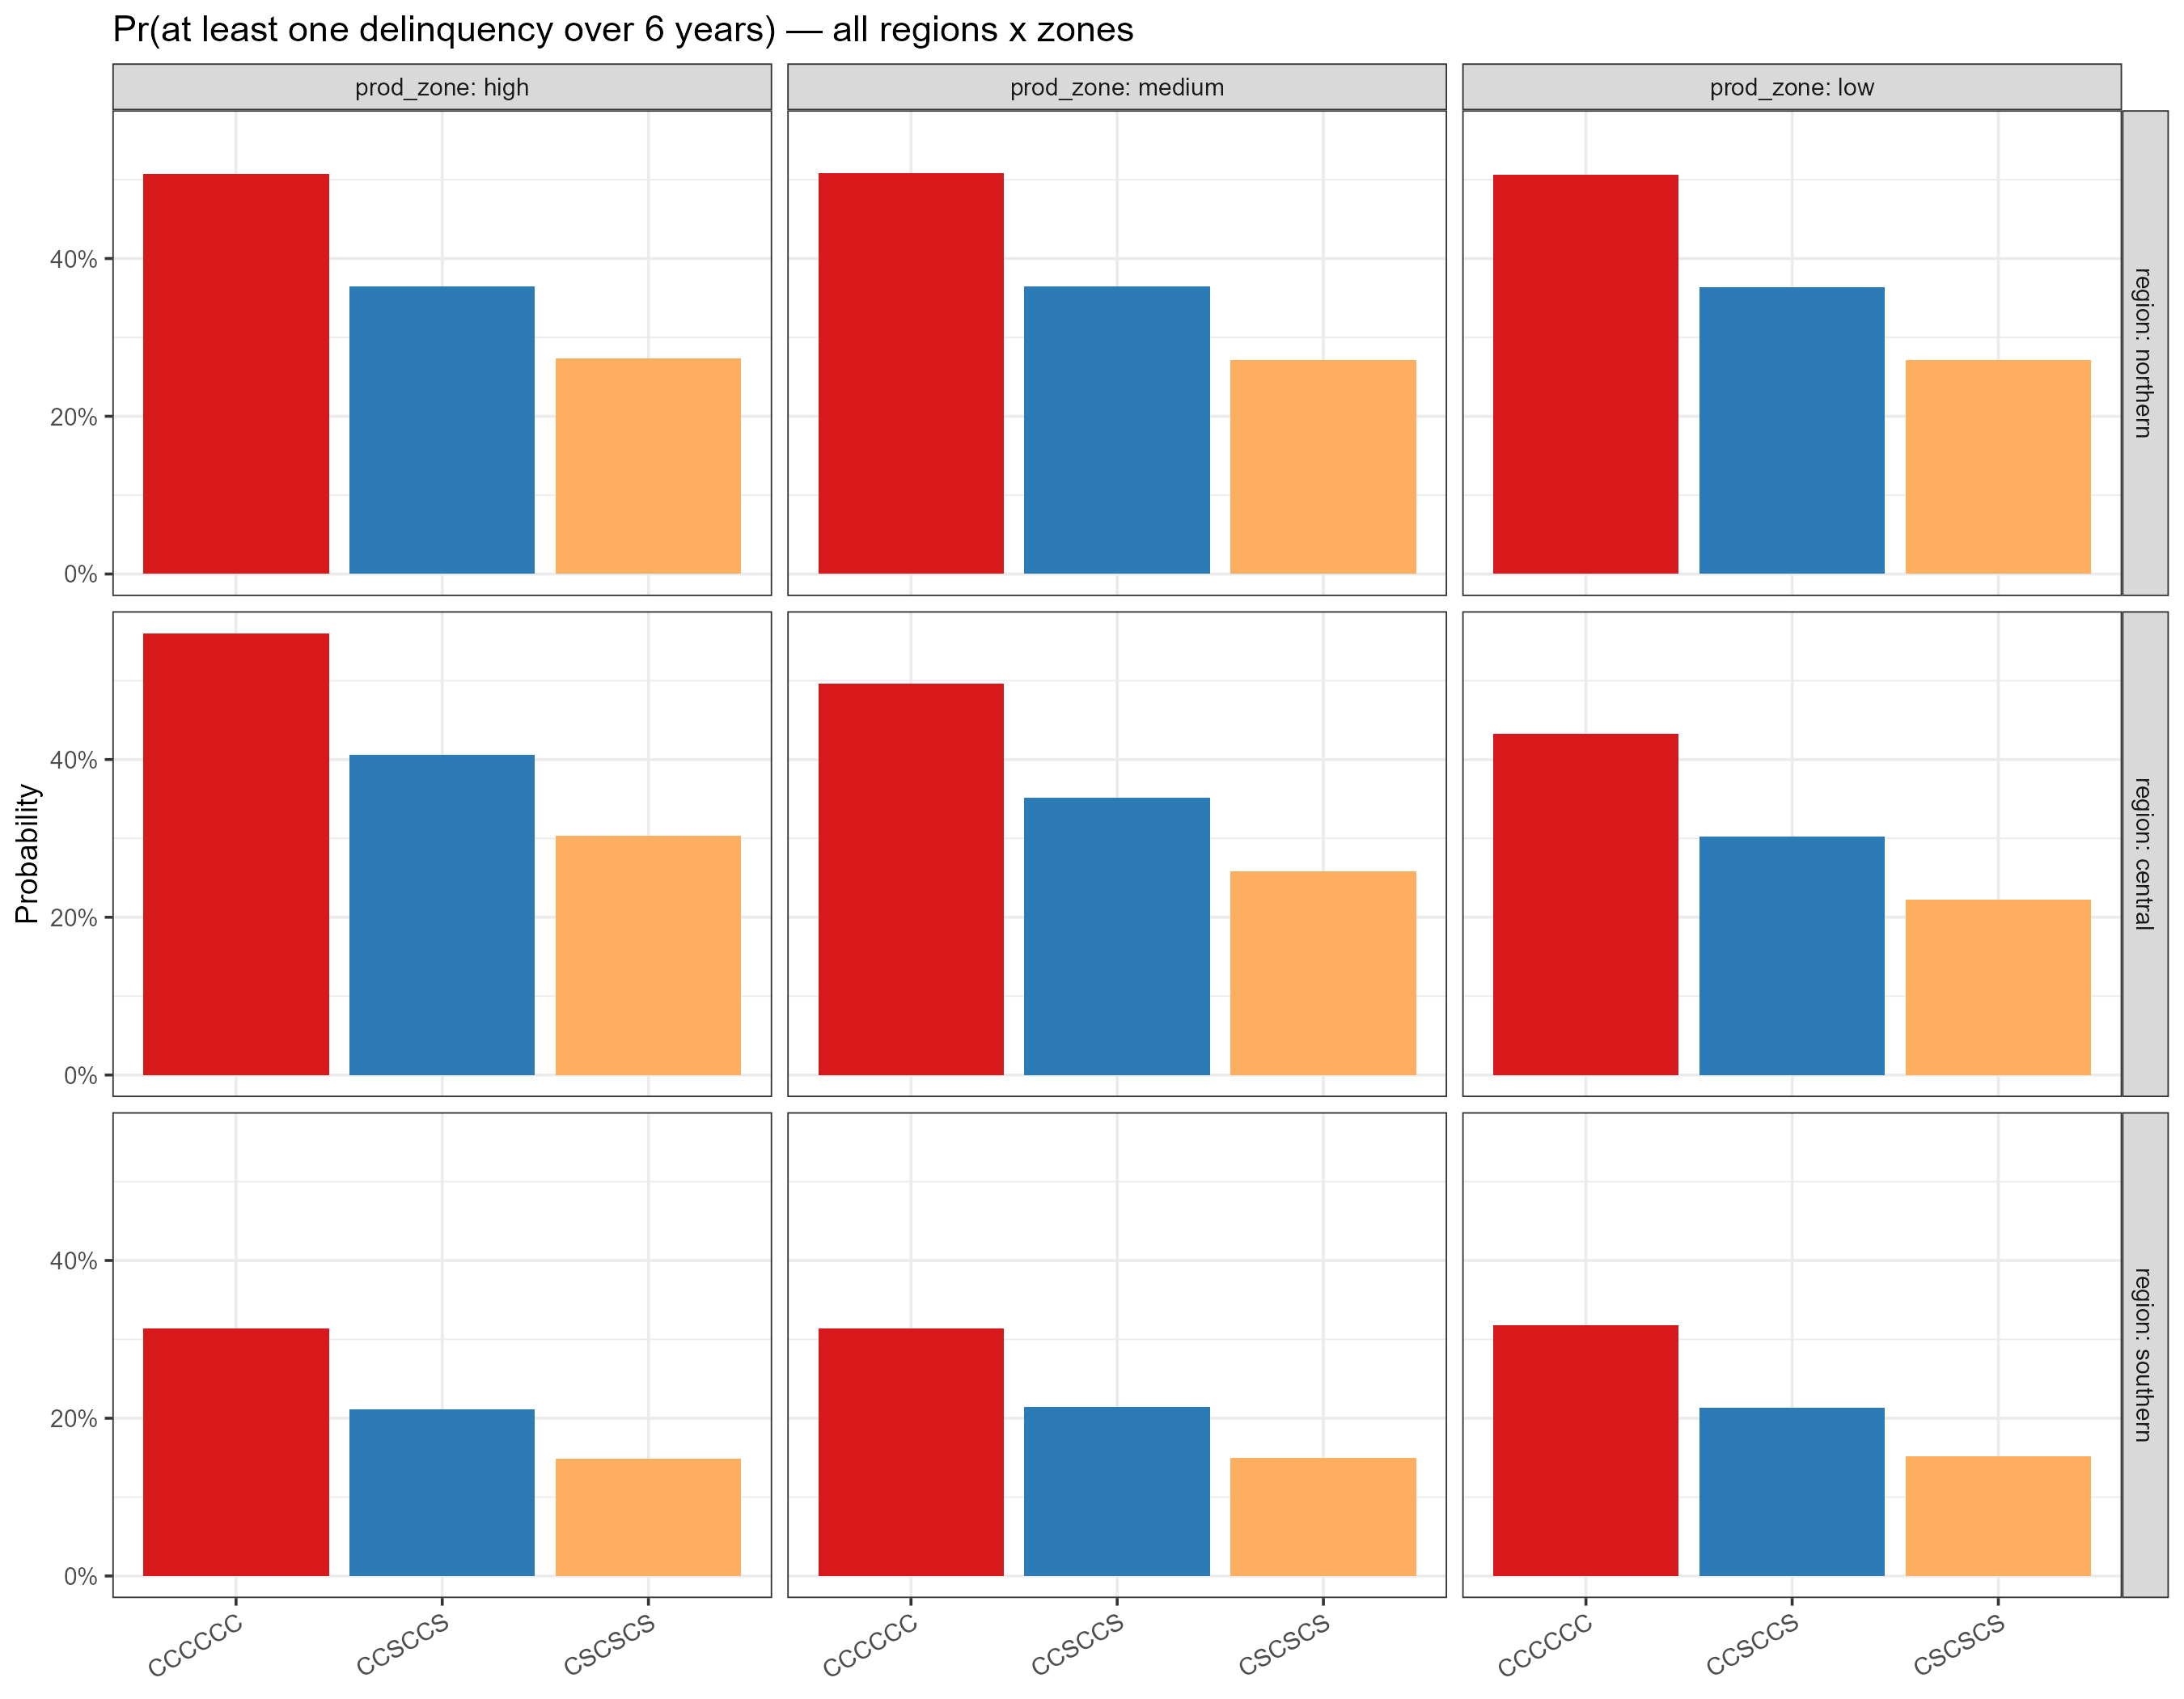
\includegraphics{figs/fig_p_bar_all.png}
}
\end{column}%
\hfill%
\begin{column}{.35\textwidth}
  \begin{wideitemize}
  \item $\approx 55\%$: \textcolor[HTML]{A50026}{Corn monoculture} (central/high)
  \item $\approx 30\%$: \textcolor[HTML]{313695}{Perfect rotation} (same cell)
  \item $-25 pp$: Risk reduction from rotating
  \end{wideitemize}
\end{column}%
\end{columns}
\end{frame}

\begin{frame}{Soy years dampen the debt cycle — the sawtooth}
\begin{columns}[T] % align columns
\begin{column}{.65\textwidth}
\resizebox{\textwidth}{!}{
  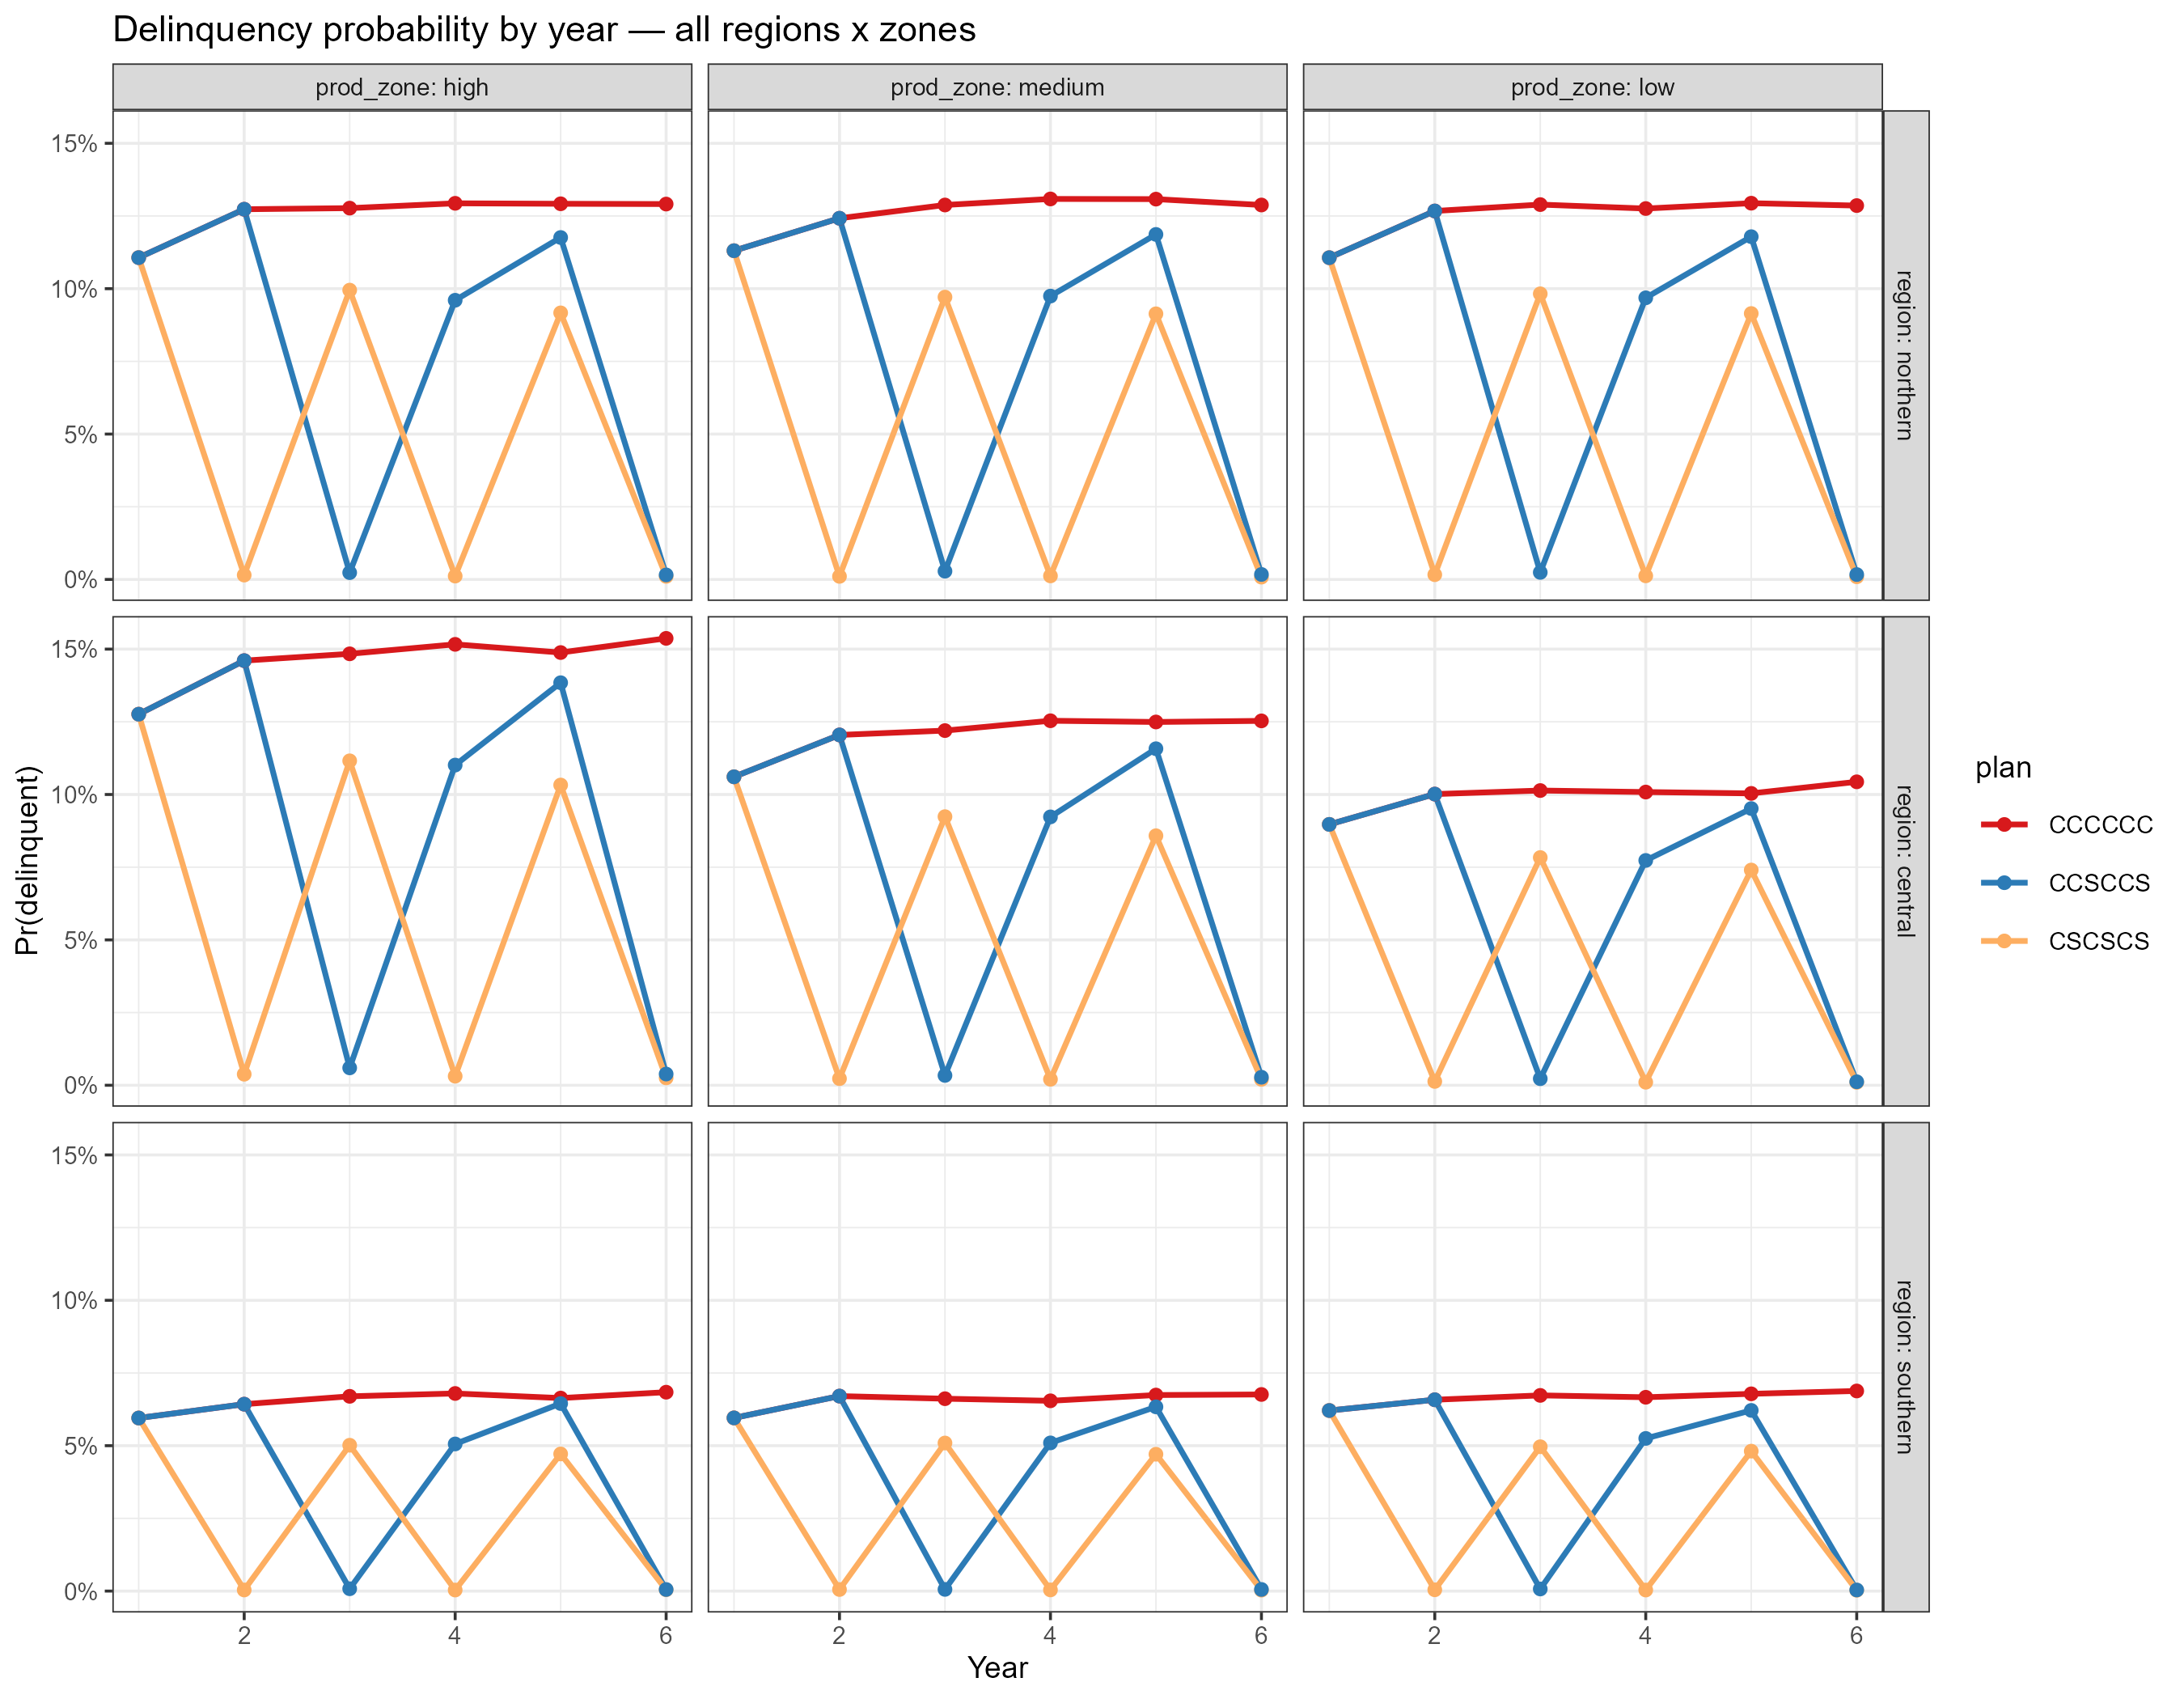
\includegraphics{figs/fig_p_year_all.png}
}
\end{column}%
\hfill%
\begin{column}{.35\textwidth}
  \begin{itemize}
  \item \textcolor{cardinalred}{Continuous corn} holds a flat elevated hazard.
  \item Rotations crash toward zero in \textcolor{green}{soy-harvest years}, then rebuild.
  \item A soy harvest \textbf{retires accumulated rollover debt}, resetting the farm to near-zero before the next corn run.
  \item However, this is a consequence of the data coming from a period where soybean returns were higher than those of corn.
  \end{itemize}
\end{column}%
\end{columns}
\end{frame}

\begin{frame}{Survival curves show where rotation pulls farms apart}
\begin{columns}[T] % align columns
\begin{column}{.65\textwidth}
\resizebox{\textwidth}{!}{
  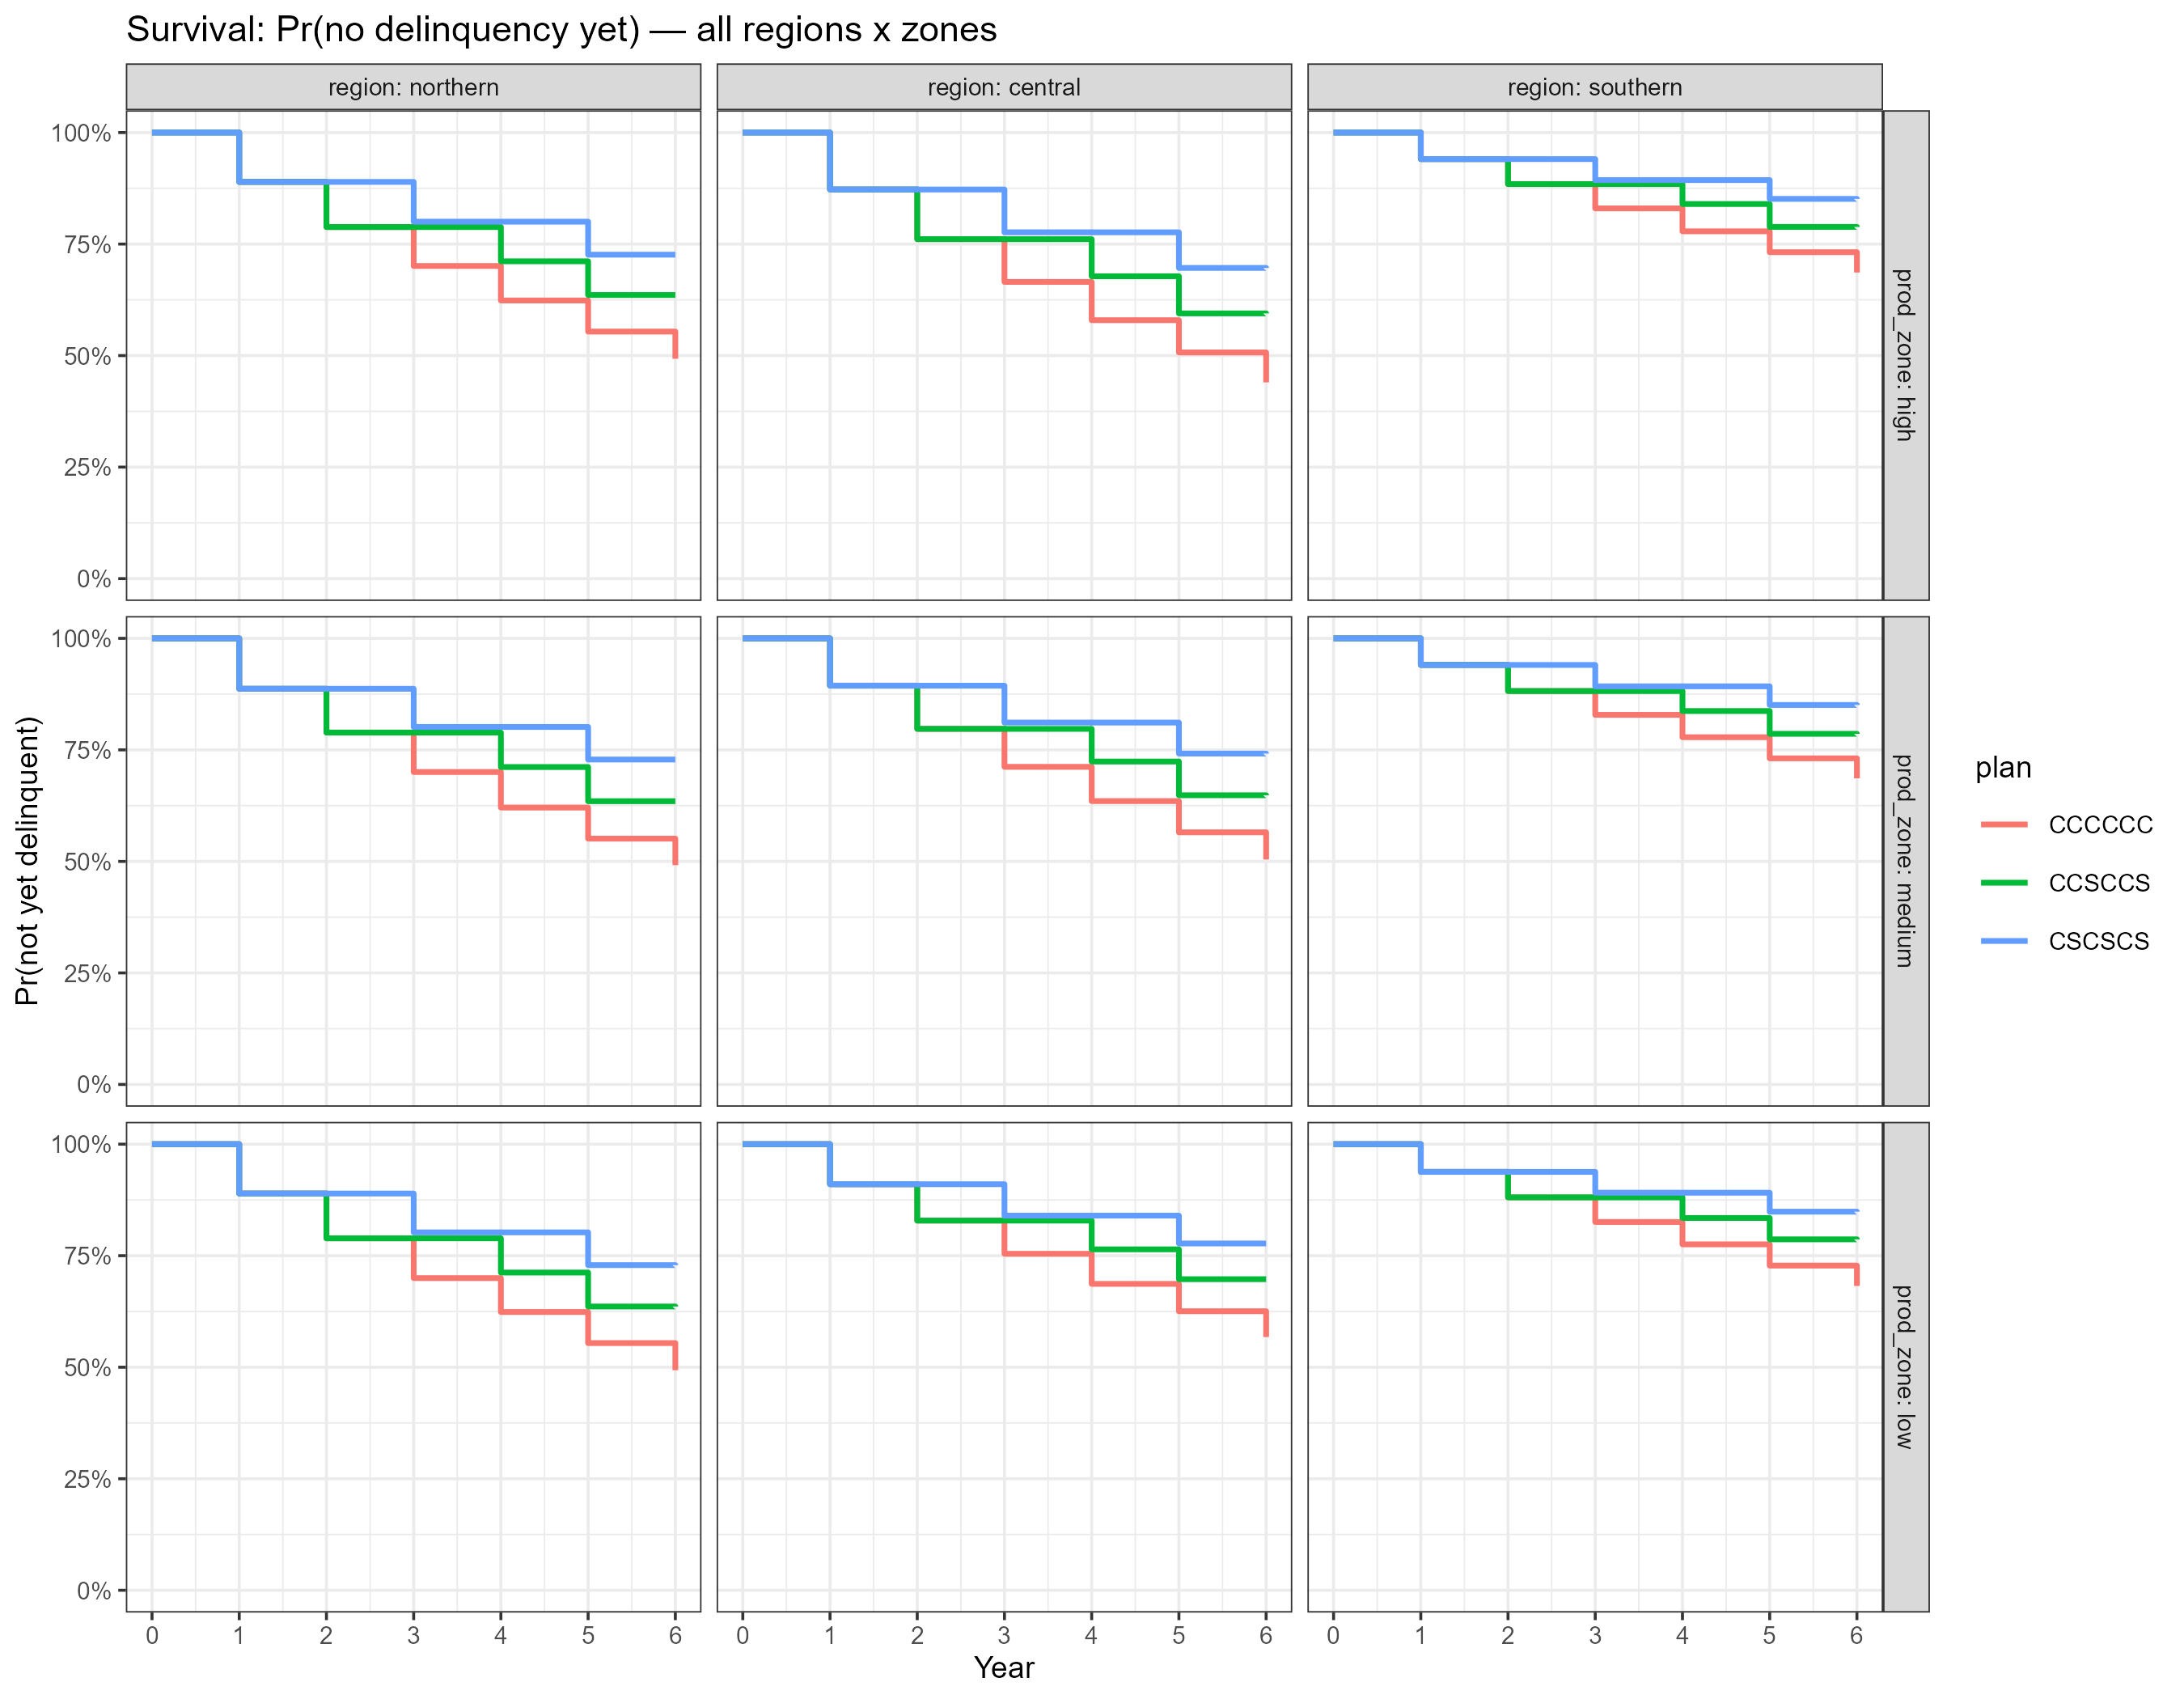
\includegraphics{figs/fig_p_surv_all.png}
}
\end{column}%
\hfill%
\begin{column}{.35\textwidth}
  \begin{itemize}
  \item Drops concentrate in corn years; soy years are flat.
  \item By year 3, the curves have already separated by 15–20 pp; the earliest events do the lasting damage.
  \item By year 6, alternation preserves 70–85\% of farms in solvency; continuous corn 45–70\%.
  \end{itemize}
\end{column}%
\end{columns}
\end{frame}

\begin{frame}{The natural hedge mostly helps continuous corn}
\begin{columns}[T] % align columns
\begin{column}{.65\textwidth}
\resizebox{\textwidth}{!}{
  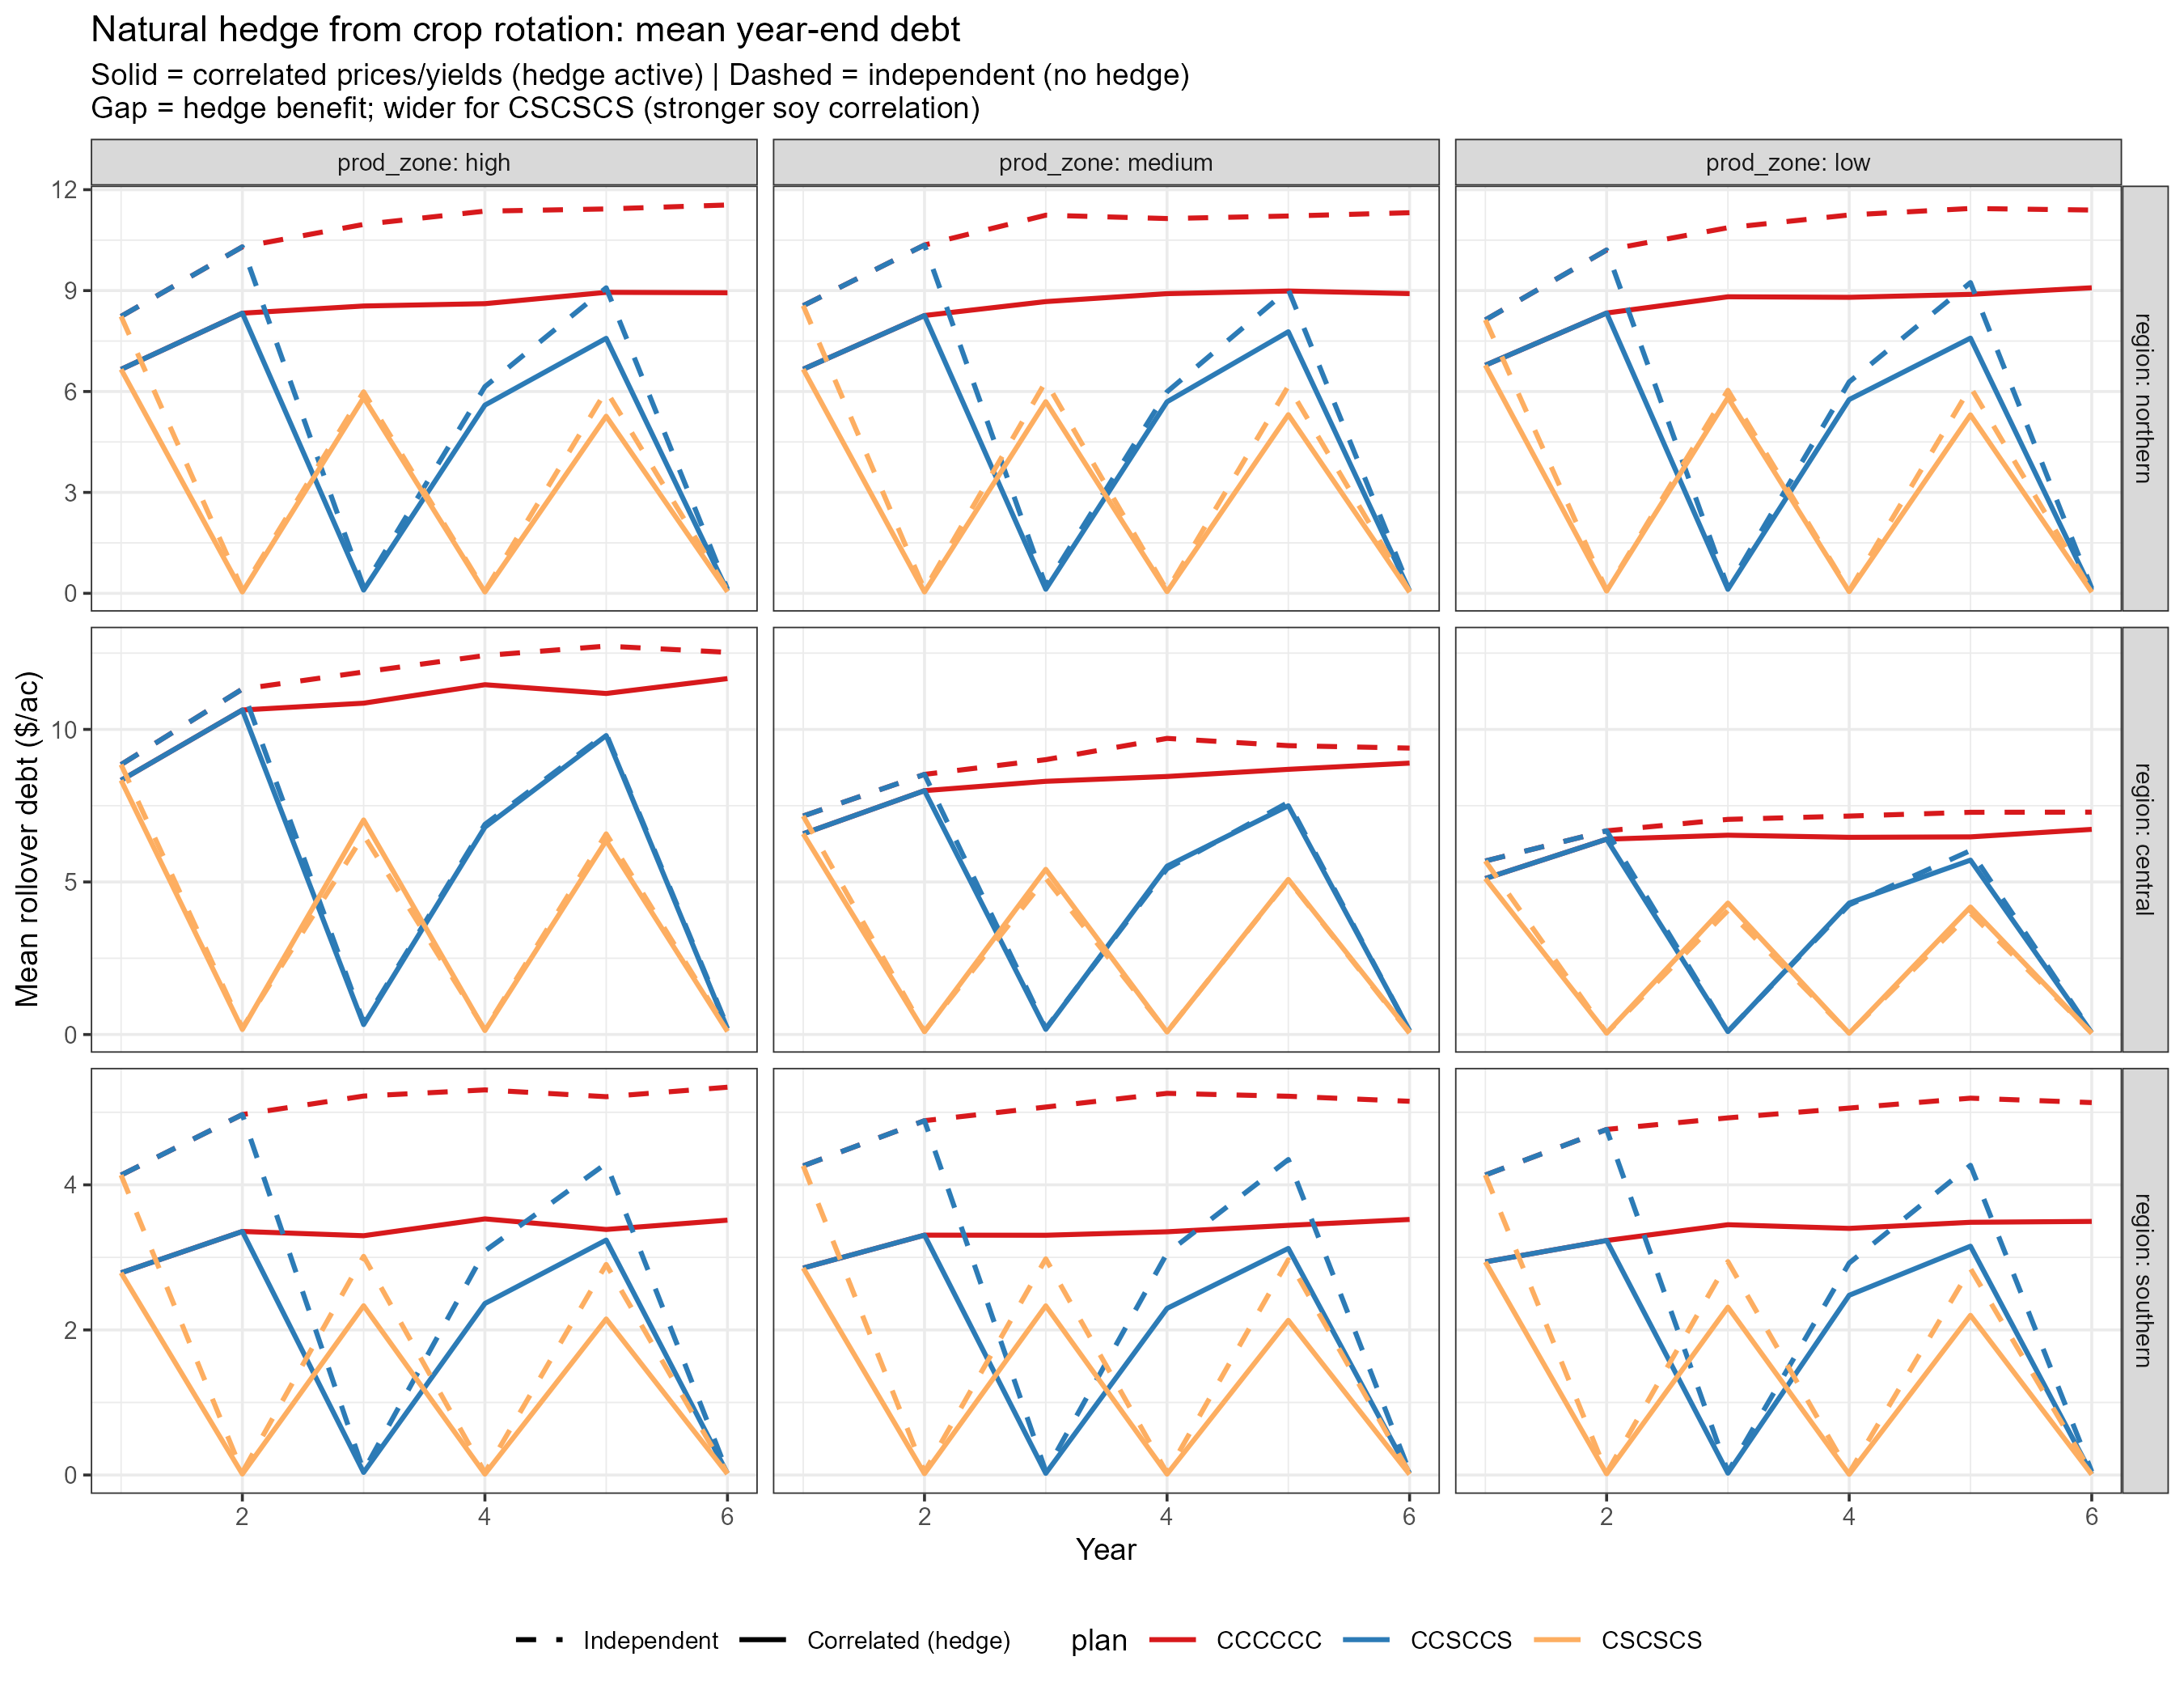
\includegraphics{figs/fig_p_debt_all.png}
}
\end{column}%
\hfill%
\begin{column}{.35\textwidth}
  \textbf{Details}:

  \textbf{Solid lines}: correlated prices/yields (hedge active).

  \textbf{Dashed lines}: independent (no hedge).

  The vertical gap is the hedge benefit.
  
  The gap is widest for \textcolor{cardinalred}{continuous corn} and nearly closes for rotations.
  
  Hedge and rotation are partial substitutes.
\end{column}%
\end{columns}
\end{frame}

\begin{frame}{Peak loan demand stays under common credit limits}
\begin{columns}[T] % align columns
\begin{column}{.65\textwidth}
\resizebox{\textwidth}{!}{
  \includegraphics{figs/fig_peak_loan_all.png}
}
\end{column}%
\hfill%
\begin{column}{.35\textwidth}
  \textbf{What this tells lenders}:
  \begin{itemize}
  \item Medians cluster near \$/ac 500–550. Rationing at the \$700, \$900, \$1,200 ceilings is rare.
  \item But rotation shifts the whole distribution down, widening the safety margin.
  \item Rotation history is an observable, verifiable risk factor lenders can price into operating-credit underwriting.
  \end{itemize}
\end{column}%
\end{columns}
\end{frame}

\begin{frame}{Shapley Decomposition}
\begin{block}{What causes delinquency?}
    \begin{itemize}
        \item Variance decomposition answers: "What share of revenue variance comes from price?" \textcolor{green}{86-89\% price, 11-14\% yield}.
        \item Shapley decomposition answers: "What share of the probability of crossing the default threshold is caused by price?" \textcolor{red}{92-100\% price}.
    \end{itemize}
\end{block}
\begin{block}{How it works}
    \begin{description}
        \item[$V(A)$]: $\Pr(delinquency)$ when sources in $A$ are stochastic, sources outside $A$ fixed at their means.
        \item[$V(\emptyset)$] Both fixed at means $\rightarrow$ baseline (zero stochastic risk).
        \item[$V(\{P\})$] Only price stochastic $\rightarrow$ Delinquency due to price only. 
        \item[$V(\{Y\})$] Only yield stochastic $\rightarrow$ Delinquency due to yield only.
        \item[$V(\{P,Y\})$] Both stochastic $\rightarrow$ full delinquency probability.
    \end{description}
    \begin{equation*}
        \phi_{P}=\frac{1}{2}\left[V(\{P\})-V(\emptyset)\right]+\frac{1}{2}\left[V(\{P,Y\})-V(\{Y\})\right]
    \end{equation*}
\end{block}
\end{frame}

\begin{frame}{Shapley Decomposition}
    \begin{figure}[ht]
        \begin{minipage}[b]{0.45\linewidth}
            \centering
            \includegraphics[scale = 0.25]{figs/fig_revenue_variance_decomp.png}
            \caption{Price dominates revenue variance}
            \label{fig:fig_revenue_variance_decomp}
        \end{minipage}
        \hspace{0.5cm}
        \begin{minipage}[b]{0.45\linewidth}
            \centering
            \includegraphics[scale = 0.3]{figs/fig_shapley_price_share.png}
            \caption{Shapley values}
            \label{fig:fig_shapley_price_share}
        \end{minipage}
    \end{figure}
\end{frame}

\begin{frame}{Price dominates revenue variance}
    \begin{wideitemize}
       \item Variance share: 86-89\% of gross revenue variance is attributable to price. 
       \item Shapley share: 96\% of gross revenue is due to price.
       \item Stable across regions, zones, and plans. 
       \item \textbf{Implication}: the natural price–yield hedge can only do so much at the field level; the dominant source of variance isn't what the correlation is between. 
       \item Yield has a physical lower bound (zero-yield is rare in Illinois). Price has no such bound; left tails are long. 
       \item The default threshold is a fixed dollar hurdle. A price draw of 30\% below the median moves revenue far more than an equal-sized yield draw.
    \end{wideitemize}
\end{frame}

%\begin{frame}{Price dominates revenue variance}
%\begin{columns}[T] % align columns
%\begin{column}{.65\textwidth}
%\resizebox{\textwidth}{!}{
%  \includegraphics{figs/fig_revenue_variance_decomp.png}
%}
%\end{column}%
%\hfill%
%\begin{column}{.35\textwidth}
%  \begin{itemize}
%  \item \textcolor{razorbackred}{86-89\% of gross revenue variance is attributable to price}.
%  \item Stable across regions, zones, and plans.
%  \item \textbf{Implication}: the natural price–yield hedge can only do so much at the field level; the dominant source of variance isn't what the correlation is between.
%  \end{itemize}
%\end{column}%
%\end{columns}
%\end{frame}

%\begin{frame}{Year-2 soy price shock moves only the soy-in-yr-2 plan}
%\begin{columns}[T] % align columns
%\begin{column}{.65\textwidth}
%\resizebox{\textwidth}{!}{
%  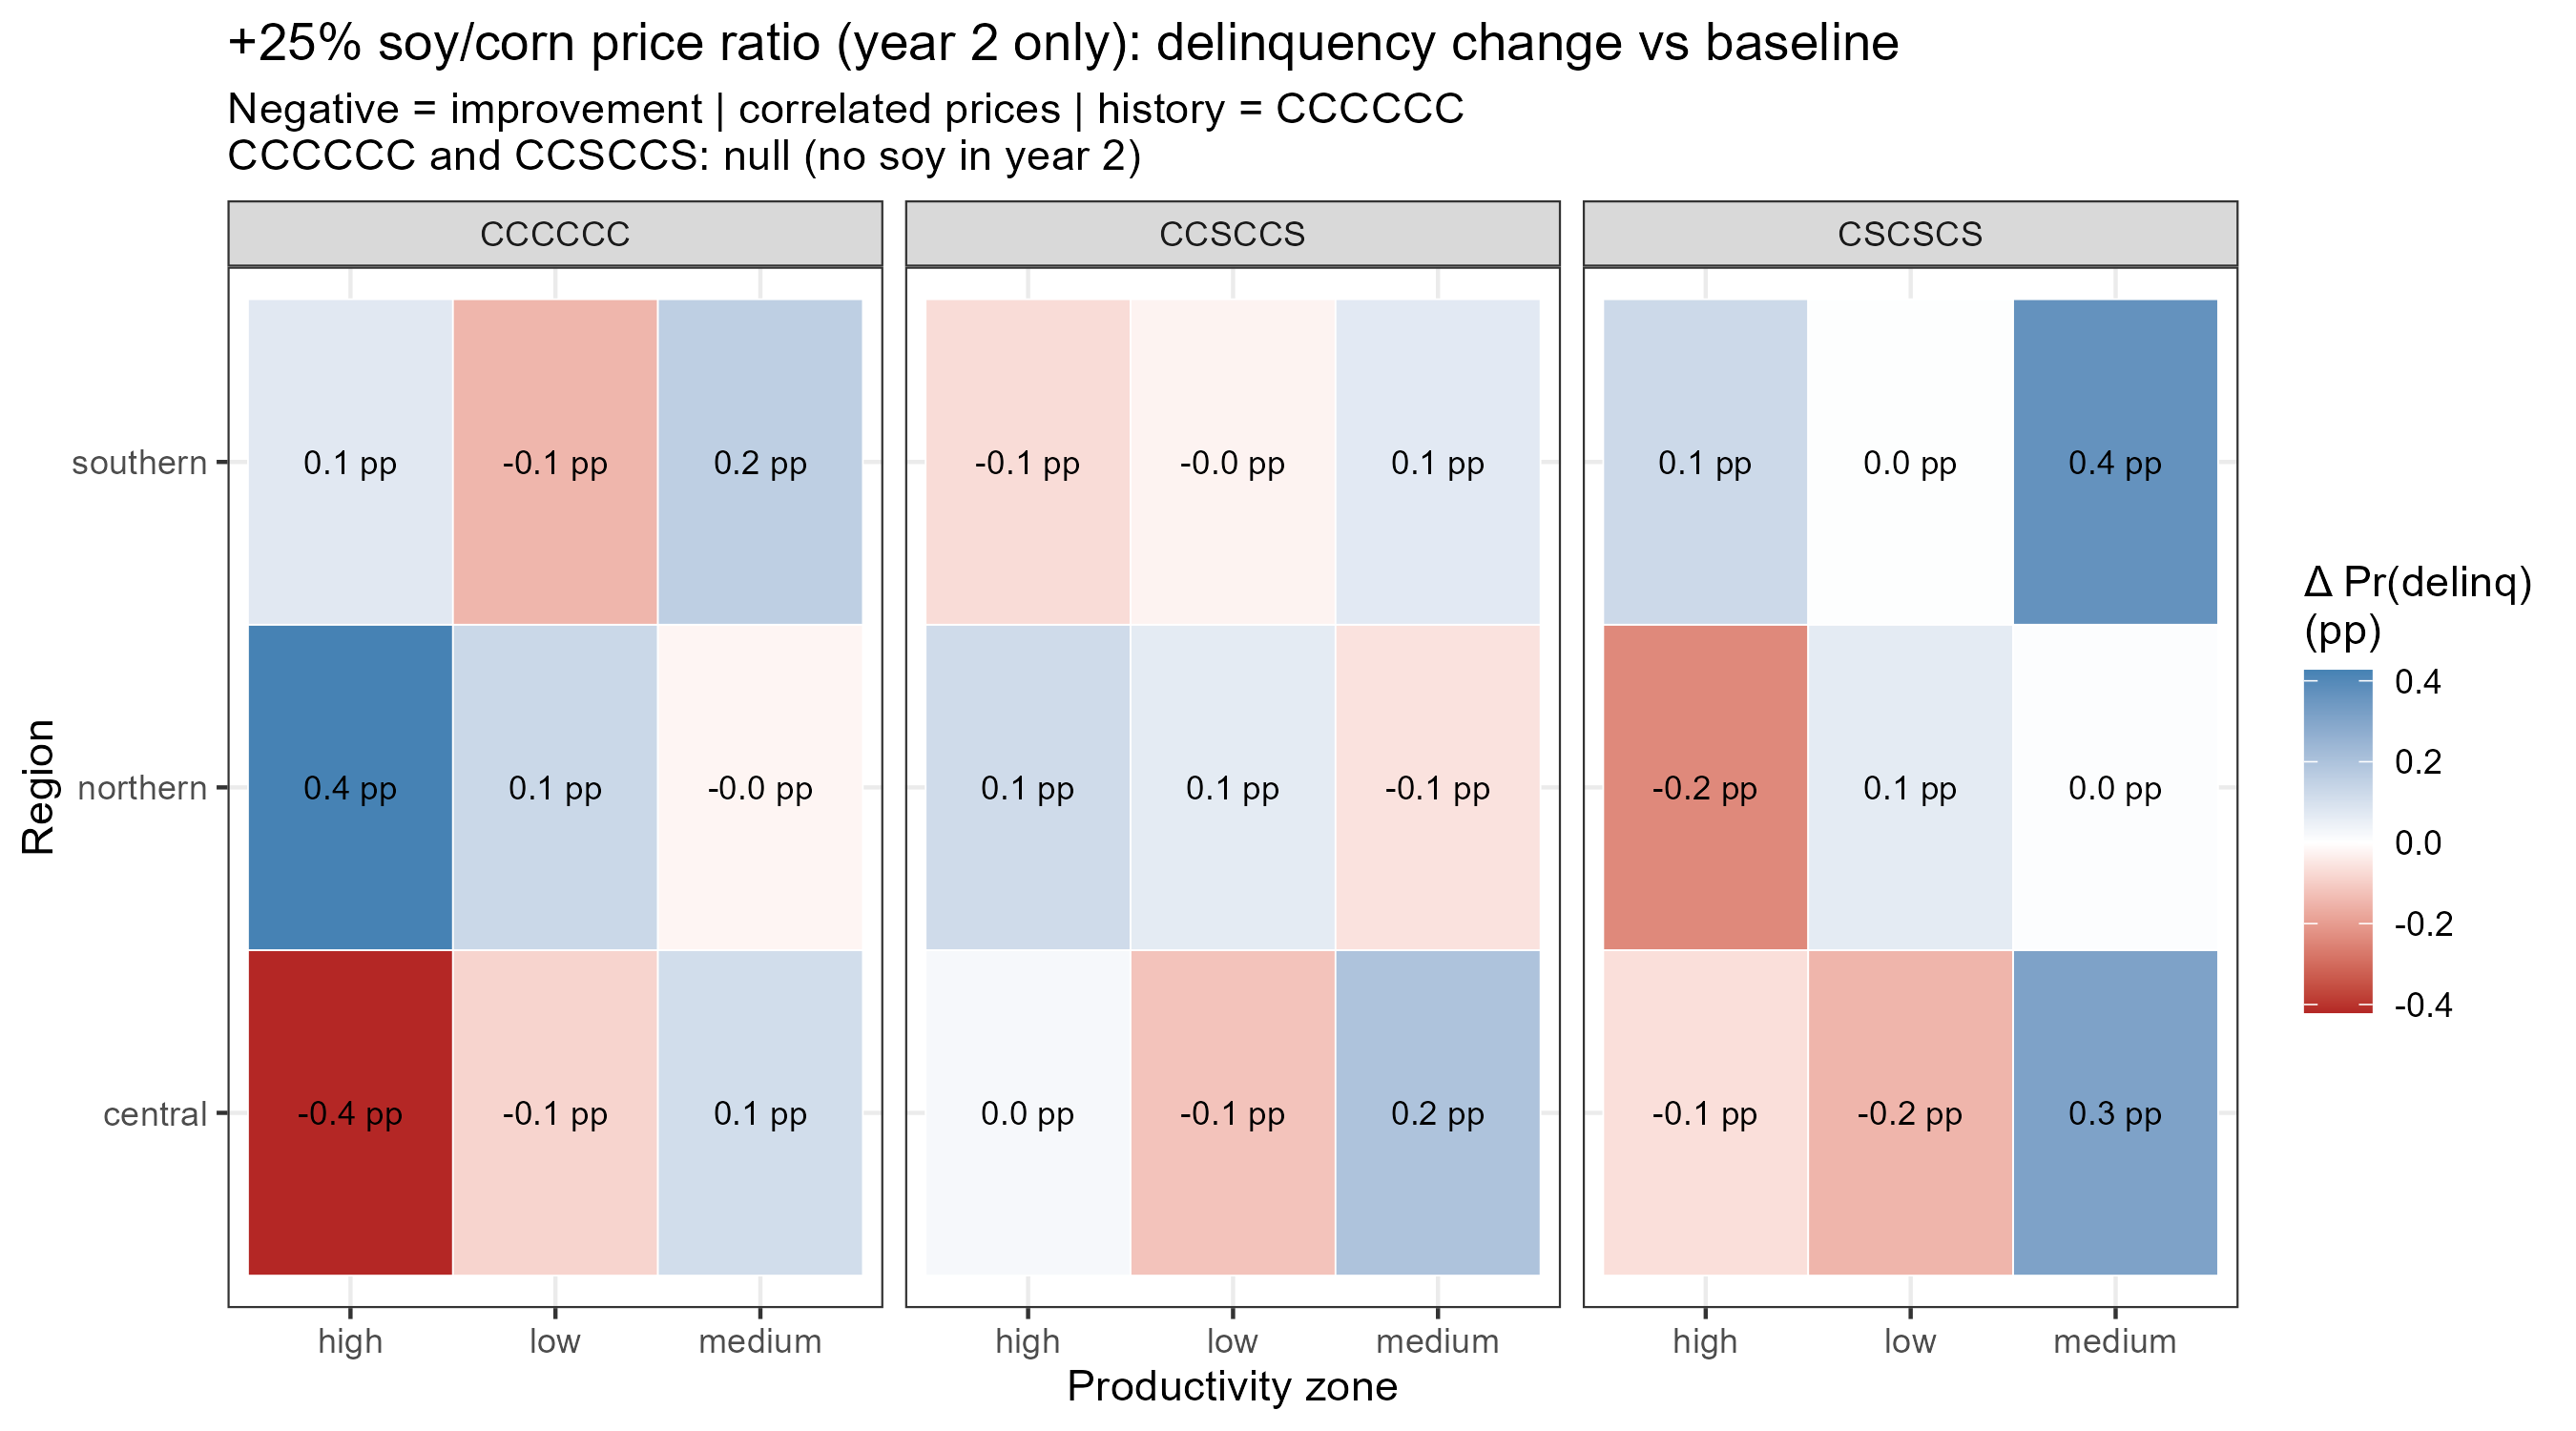
\includegraphics{figs/fig_price_sensitivity_soy_yr2.png}
%}
%\end{column}%
%\hfill%
%\begin{column}{.35\textwidth}
%\begin{itemize}
%    \item This is a kind of placebo
%    \item $+25\%$ soy/corn price ratio in year 2 only.
%    \item CCCCCC and CCSCCS plant no soy in year 2 $\rightarrow$ null.
%    \item CSCSCS plants soy in year 2 $\rightarrow$ responds.
%    \item Nulls validate the cash-flow mechanism, not an aggregate price effect.
%\end{itemize}
%\end{column}%
%\end{columns}
%\end{frame}

\begin{frame}{Implications}
\begin{block}{Lenders}
    \textbf{Rotation history is a credit-risk factor}

    Two farms with identical balance sheets but different 6-year rotation states face delinquency probabilities that differ by a factor of 2+.
\end{block}

\begin{block}{Insurers}
    \textbf{Single-year products misprice multi-year exposure}

    Revenue protection calibrated to single-year loss ratios systematically understates ruin risk for corn-heavy producers — the APH baseline doesn't account for the rollover channel.
\end{block}

\begin{block}{Extension}
    \textbf{Financial case reinforces the agronomic one}

    Rotation's soil-health benefits are matched by a balance-sheet benefit. The financial argument is independent of the agronomic one and additive to it.
\end{block}
\end{frame}

\begin{frame}{Takeaways}
\begin{block}{Key figures}
    \begin{itemize}
        \item Rotation cuts delinquency by as much as 25pp.
        \item 92-100\% of total delinquency risk comes from price uncertainty.
        \item By year 3, the gap between CCCCCC and CSCSCS is already 15–20 percentage points.
    \end{itemize}
\end{block}
\begin{block}{Three things to remember}
    \begin{enumerate}
        \item \textcolor{razorbackred}{Rotation cuts multi-year delinquency through periodic debt resets}.
        
        The mechanism is the soy-year sawtooth, not yield smoothing.
        \item \textcolor{springwater}{Price uncertainty dominates both revenue variance and delinquency causation}.

        The natural hedge is modest and largely redundant where rotation operates.
        \item \textcolor{pine}{Rotation history is a missing variable in credit-risk and crop-insurance models}.

        Observable, verifiable, predictive — and absent from current practice.
    \end{enumerate}
\end{block}
\end{frame}

\begin{frame}{}
	\centering \Huge
	\emph{Thank You!}
\end{frame}

\begin{frame}[allowframebreaks]{References}
	\bibliography{references.bib}	
\end{frame}	


\end{document}